\documentclass[../main.tex]{subfiles}

\begin{document}
Si vuole qui dare un esempio di come una matrice Laplaciana venga realmente costruita e una breve analisi degli autovalori.
Si consideri come primo esempio il network completamente connesso rappresentato in Fig. \ref{fig:network_connesso}.
\begin{figure}[H]
    \centering
    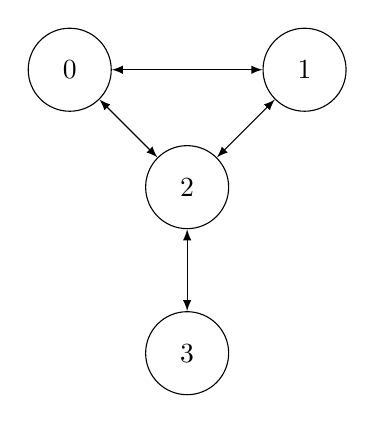
\begin{tikzpicture}[>=latex,every node/.style={draw,circle,minimum width={3em},node distance=6em}]
    \node (2) {2};
    \node [above left of=2] (0) {0}; 
    \node [above right of=2] (1) {1};
    \node [below of=2] (3) {3};  
    \draw [<->] (2) -- (0);
    \draw [<->] (2) -- (1);
    \draw [<->] (0) -- (1);
    \draw [<->] (2) -- (3);
    \end{tikzpicture}
    \caption[Grafo di un network connesso]{\emph{Esempio network connesso.}}
    \label{fig:network_connesso}
\end{figure}
Questo \`e descritto dalla matrice di adiacenza:
\begin{equation}
    \mathcal{A}=\left(
    \begin{matrix}
        0 & 1 & 1 & 0\\
        1 & 0 & 1 & 0\\
        1 & 1 & 0 & 1\\
        0 & 0 & 1 & 0
    \end{matrix}\right)
\end{equation}
La matrice Laplaciana costruita dalla definizione risulta
\begin{equation}
    \mathcal{L}=\left(
    \begin{matrix}
        2 & -1 & -1 & 0\\
        -1 & 2 & -1 & 0\\
        -1 & -1 & 3 & -1\\
        0 & 0 & -1 & 1
    \end{matrix}\right)
\end{equation}
la quale possiede autovalori 0, 1, 3, 4.
In particolare, si nota la presenza dell'autovalore nullo, come previsto teoricamente.\\
Si esegua ora la stessa analisi per un network disconnesso, come quello in Fig. \ref{fig:network_sconnesso}.
\begin{figure}[H]
    \centering
    \begin{tikzpicture}[>=latex,every node/.style={draw,circle,minimum width={3em},node distance=6em}]
    \node (0) {0};
    \node [above right of=0] (1) {1}; 
    \node [below right of=1] (2) {2};
    \node [right of=2] (3) {3};
    \node [below right of=3] (4) {4};
    \node [above right of=4] (5) {5};
    \draw [<->] (0) -- (1);
    \draw [<->] (1) -- (2);
    \draw [<->] (3) -- (4);
    \draw [<->] (4) -- (5);
    \draw [<->] (3) -- (5);
    \end{tikzpicture}
    \caption[Grafo di un network sconnesso]{\emph{Esempio network sconnesso.}}
    \label{fig:network_sconnesso}
\end{figure}
La matrice di adiacenza \`e
\begin{equation}
    \mathcal{A}=\left(
    \begin{matrix}
        0 & 1 & 0 & 0 & 0 & 0\\
        1 & 0 & 1 & 0 & 0 & 0\\
        0 & 1 & 0 & 0 & 0 & 0\\
        0 & 0 & 0 & 0 & 1 & 1\\
        0 & 0 & 0 & 1 & 0 & 1\\
        0 & 0 & 0 & 1 & 1 & 0\\
    \end{matrix}\right)
\end{equation}
La matrice Laplaciana in questo caso diviene
\begin{equation}
    \mathcal{L}=\left(
    \begin{matrix}
        1 & -1 & 0 & 0 & 0 & 0\\
        -1 & 1 & -1 & 0 & 0 & 0\\
        0 & -1 & 1 & 0 & 0 & 0\\
        0 & 0 & 0 & 2 & -1 & -1\\
        0 & 0 & 0 & -1 & 2 & -1\\
        0 & 0 & 0 & -1 & -1 & 2\\
    \end{matrix}\right)
\end{equation}
ed ha autovalori 0, 0, 1, 2, 3, 3.
Anche in questo caso vi sono due autovalori nulli, essendo il network sconnesso, come previsto dalla teoria.